\begin{tcolorbox}[
    colback=green!5!white, % Very light red background (5% red, 95% white)
    colframe=darkgreen!40!white, % Light red border (30% red, 70% white)
   title=Motivation, % Optional title
    fonttitle=\bfseries % Bold title
    ]
    
    Analyse the macroeconomic dynamics over time:
    \begin{itemize}
        \item What are consequences of epidemic shocks?
        \item How does capital accumulation affect the distribution of income? 
    \end{itemize}
    The model features \textbf{intertemporal choices} and \textbf{economic shocks}. Limits: No heterogeneity; No shifts in employment
\end{tcolorbox}


\subsection{Households}
\subsubsection{Households: Setup}
Mass of one identical and infinitely lived households:
\begin{itemize}
    \item $x(i)$ denotes income of household $i\in[0;1]$ $\rightarrow$ Aggregate income: $X=\int_0^1x(i)di$
    \begin{itemize}
        \item Identical households: $x(i)=\bar{x}\quad \forall \space i$ $\Longrightarrow$ $X=\int_0^1x(i)di=\int_0^1\bar{x}di=\bar{x}$ 
        \begin{figure}[H]
            \centering
            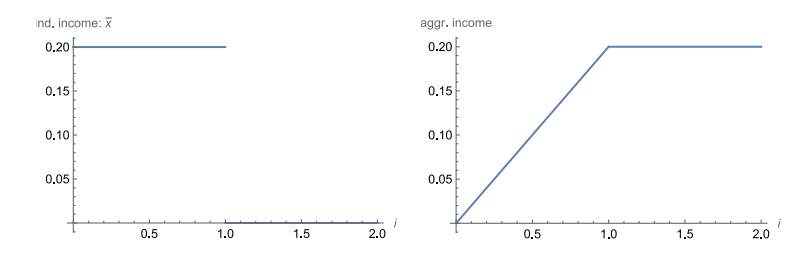
\includegraphics[width=0.6\linewidth]{hhincome.png}
            \caption{Individuals and aggregate income with mass one identical households}
        \end{figure}
        \scriptsize{Note: If mass of households was 2 instead of 1 the aggregate income would be $2\bar{x}$ and there would be twice as much individuals}
    \end{itemize}
    \item $L$ denotes households members who all supply one unit of time $\rightarrow$ Aggregate labor supply = $L*1$
    \begin{itemize}
        \item $L$ is fully inelastic (vertical line in w - L graph) and theoretically could also change over time, i.e. $L(t)$
    \end{itemize}
    \item $a(t)$ denotes wealth which is lent to firms
    \item Quantities per household coincide with aggregate quantities
    \item Household income ( = aggregate income): $X(t)=w(t)L+r(t)a(t)$ \textit{($r:$ interest rate; $w:$ wage rate; $t\in[0,\infty]$ time)}
\item Every household is assumed to \textbf{maximize its life-time utility}\\
$$U = \int_{0}^{\infty} u\big[C(t)\big] \cdot e^{-\rho t} \, dt \quad \text{with} \quad \rho > 0$$
whereas $\rho$ is the time preference rate, $u$ is the instant utility, $C$ is consumption
\end{itemize}
The higher $\rho$, the faster $e^{-pt}$ converges to zero: 
\begin{figure}[h]
\centering
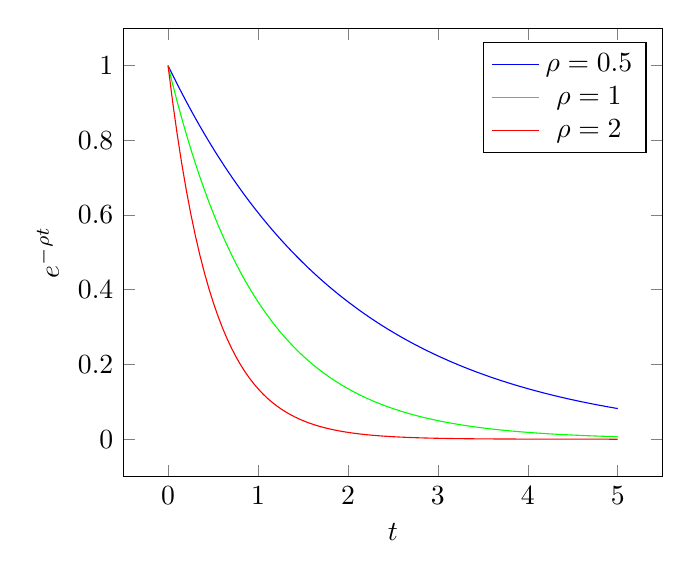
\begin{tikzpicture}
\begin{axis}[
    xlabel={$t$},
    ylabel={$e^{-\rho t}$},
    legend pos=north east,
    domain=0:5,
    samples=100,
    cycle list name=color list,
]
\addplot[no markers, blue] {exp(-0.5*x)};
\addlegendentry{$\rho=0.5$}

\addplot[no markers, green] {exp(-1*x)};
\addlegendentry{$\rho=1$}

\addplot[no markers, red] {exp(-2*x)};
\addlegendentry{$\rho=2$}
\end{axis}
\end{tikzpicture}
\end{figure}
\subsubsection{Households: Instantaneous utility}

Households have the instantaneous utility function \textit{(Instantaneous means that the utility function describes satisfaction at a single moment, not aggregated over a period)}: 
$$u\big[C(t)\big] = \frac{C(t)^{1-\sigma} - 1}{1 - \sigma} \quad \text{with} \quad \sigma > 0$$

Alternative formulation \textit{(as $\ \lim_{\sigma \to 1} u(C)=ln(C)$)}:
$$u(C) =
\begin{cases}
\frac{C^{1-\sigma}}{1-\sigma} & \text{for } \sigma \neq 1 \\
\ln(C) & \text{for } \sigma = 1
\end{cases}$$
\begin{itemize}
    \item $u$ is compatible with steady state growth 
    \item Life-time utility (welfare) functions implies CIES: constant intertemporal elasticity of substitution 
    \item Elasticity of marginal utility w.r.t. C \textit{( $\rightarrow$ $C$ is increased by 1\%, how does $u'(C)$ change?)} is constant: 
$$
\eta_{u'(C),C} := \frac{du'(C)/u'(C)}{dC/C} = \frac{du'(C)/dC \cdot C}{u'(C)} = \frac{\textcolor{blue}{u''(C)} \cdot C}{\textcolor{red}{u'(C)}} =\frac{\textcolor{blue}{-\sigma C^{-\sigma-1}}*C}{\textcolor{red}{C^{-\sigma}}}=-\sigma < 0
$$
The elasticity is the relative change in $u'$ divided by the relative change in $C$.
\textit{\scriptsize{Note: The time index is suppressed}}
\end{itemize}
The \textbf{parameter $\sigma$ is a measure for concavity} of the utility function: The higher $\sigma$, the more concave is $u(C)$
\begin{figure}[H]
    \centering
    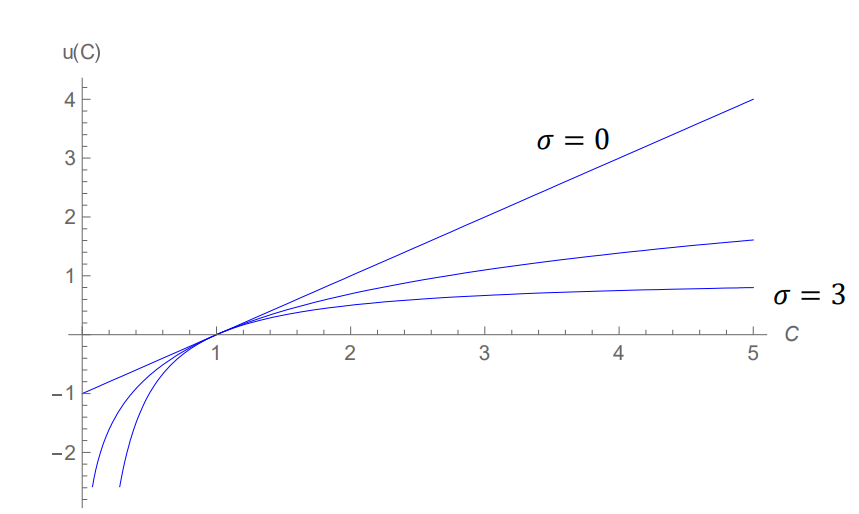
\includegraphics[width=0.5\linewidth]{instantutility.png}
    \label{fig:placeholder}

\end{figure}
\begin{itemize}
    \item $\sigma = 0 \longrightarrow$ marginal utility does not change with consumption, i.e. $u(C)$ is a straight line
    \begin{itemize}
        \item Infinite willingness to substitute consumption intertemporally
        \item Consumer is indifferent between different consumption profiles (apart from discounting with $e^{-pt}$ in lifetime utility function)
    \end{itemize}
    \item $\sigma > 0 \longrightarrow$ marginal utility declines with consumption: $u(C)$ is concave $\rightarrow$ Desire to smooth consumption over time
\end{itemize}

\begin{tcolorbox}[
    colback=blue!5!white, % Very light red background (5% red, 95% white)
    colframe=blue!40!white, % Light red border (30% red, 70% white)
    title=Example: Life-time utility over three periods, % Optional title
    fonttitle=\bfseries % Bold title
    ]
    Which consumption profile is preferable: the red or the blue one?
    \begin{figure}[H]
        \centering
        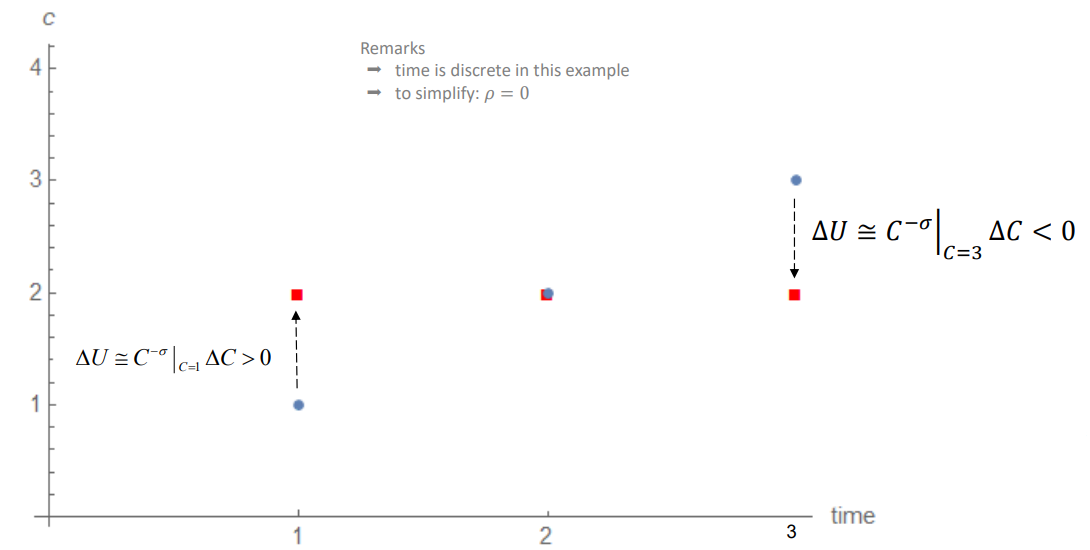
\includegraphics[width=0.5\linewidth]{lifetimeconsum.png}
    \label{fig:placeholder}
    \end{figure}
    \begin{itemize}
        \item The red consumption profile is preferable as it smoothens consumption over time compared to the blue profile.
        \item Marginal utility is given by: $u'(C)=C^{-\sigma}$ and thus, is decreasing in $C$. The more concave the utility function the higher the incentive for consumption smoothing.
        \item In the blue profile consumption at $t=3$ is $C=3$ and at $t=1$ it is $C=1$; Thus we have $u'(3)<u'(1)$\\ $\rightarrow $ Decreasing consumption in $t=3$ by $1$ and increasing consumption in $t=1$ by $1$ increases life-time utility
    \end{itemize}
\end{tcolorbox}

\subsubsection{Households: Dynamic optimization problem}
Each household solves the following problem to optimize welfare / life-time utility: 
\[
\max_{\{C(t)\}} \int_{0}^{\infty} \frac{C(t)^{1-\sigma} - 1}{1 - \sigma} e^{-\rho t} dt
\]
\[
\text{s.t. } \dot{a}(t) = w(t)L + r(t)a(t) - C(t)
\]
\begin{itemize}
    \item Initial condition: $a(0) = a_0$
    \item Terminal condition (no ponzi game condition): $\lim_{t \to \infty} e^{-R(t)} a(t) \geq 0$
    \item We have one control variable $C(t)$, and one state variable $a(t)$
    \item The control variable is chosen by the household, the state variable depends on the control variable. While the control variable can be freely chosen and could theoretically jump, the state variable does not and is more inert \textit{(träge)}.
    \item The \textit{flow budget constraint} is a \textbf{first order, linear, differential equation}. 
\end{itemize}
\\
We set up the \textbf{Hamiltonian function} for our optimization problem:
$$H := \underbrace{\frac{C^{1-\sigma} - 1}{1 - \sigma}}_{\substack{\text{instantaneous objective} \\ \text{function}}} + \underset{\substack{\text{current value} \\ \text{shadow price}}}{\lambda} \quad \underbrace{(wL + ra - C)}_{\substack{\text{RHS of dynamic} \\ \text{constraint}}}$$
First order conditions (Note that (4) is taken as given here, general form is: $\dot{\lambda}+\frac{\partial H}{\partial x}=\rho \lambda$): 
\begin{align}
    \frac{\partial H}{\partial C} &= C^{-\sigma} - \lambda = 0 \tag{3} \\[10pt]
    \dot{\lambda} &= -\frac{\partial H}{\partial a} + \rho \lambda = -\lambda r + \rho \lambda \tag{4} \\[10pt]
    \lim_{t \to \infty} &\underbrace{e^{-\rho t} \lambda(t)}_{\substack{\text{present-value} \\ \text{shadow price}}} a(t) = 0 \tag{TVC}
\end{align}
\begin{itemize}
    \item The TVC states that present value of wealth, valued at shadow price $\lambda(t)$, at infinite time must approach zero
\end{itemize}
\textbf{Keynes-Ramsey rule (KRR)} of optimal consumption: $\hat{C}:=\frac{\dot{C}}{C}=\frac{1}{\sigma}(r-\rho)$
\\Growth rate $\hat{C} > 0$, whenever $r>\rho$
\begin{itemize}
        \item \textbf{The interest rate $r$} is the premium the household receives for reducing $C$ today by $1$ unit and increasing it tomorrow by $1$ unit, i.e. $r$ is the opportunity cost of consumption today. \textbf{Higher r gives incentive to postpone C} so that higher level of $C$ can be financed tomorrow. 
        \item \textbf{The time preference rate $\rho$} is the premium the household demand to be marginally indifferent between $C$ today and tomorrow. \textbf{High $\rho$ captures impatience and reduces $C$}, i.e. the household wished to consume today rather than tomorrow.
        \item \textbf{The intertemporal elasticity of substitution $\sigma$ }captures the households willingness to substitute consumption intertemporally. Small $\sigma$ implies that $u'(C)$ does not fall strongly as $C$ increases, i.e. the household has a high willingness to substitute consumption intertemporally and $r>\rho$ unfolds strong incentives to substitute consumption intertemporally
    \end{itemize}
$\longrightarrow$ If $r >\rho$ it seems rational to postpone consumption into the future; The smaller $\sigma$, the stronger does this incentive unfold.

\paragraph{Note on macroeconomic equilibrium:}
Steady state implies that $c:=\frac{C}{Y}$ remains constant, hence $\hat{C}=\hat{Y}$ in the long run. KRR demonstrates that $r$ plays prominent role in determining $\hat{C}$ and thus $\hat{Y}$. As $r=F'(K)-\delta$ anything that affects $F'(K)$ (MPK) impacts the growth rate. If $F'(K)>0$ and $F''(K)<0$ MPK diminishes as capital is being accumulated until $r=\rho$. Economic growth is, then, only possible if $F'(K)-\delta>\rho$.


\begin{tcolorbox}[
    colback=red!5!white, % Very light red background (5% red, 95% white)
    colframe=red!40!white, % Light red border (30% red, 70% white)
    title=Derivation of the Keynes-Ramsey rule (KRR), % Optional title
    fonttitle=\bfseries % Bold title
    ]
Take equation (3), rearrange and differentiate (chain rule!): 
$$\frac{d}{dt}(C^{-\sigma}) = \frac{d}{dt}(\lambda) \quad \Leftrightarrow \quad -\sigma C^{-\sigma - 1} \dot{C} = \dot{\lambda}$$
Plug in (4) 
$$ -\sigma C^{-\sigma - 1} \dot{C} = -\lambda r+\rho \lambda $$
Divide by $C^{-\sigma}=\lambda$ (3):
$$ \frac{-\sigma C^{-\sigma - 1} \dot{C}}{C^{-\sigma}} = \frac{-\lambda r+\rho \lambda}{\lambda}$$
Rearrange:
$$-\sigma C^{- 1} \dot{C} = - r+\rho $$
$$\hat{C}=\frac{\dot{C}}{C}=\frac{1}{\sigma}(r-\rho)$$
Another method would be to take $ln$ of equation $(3)$ and take the derivative.
\end{tcolorbox}


\subsubsection{Households: Reduced form of the Ramsey model}
The reduced form of the Ramsey model comprises two linear differential equations in \(c(t)\) and \(a(t)\) with time-varying coefficients:

\begin{align}
    \dot{c}(t) &= c(t) \frac{r(t) - \rho}{\sigma} \label{eq:c_dot} \\
    \dot{a}(t) &= r(t)a(t) + w(t) - c(t) \label{eq:a_dot}
\end{align}


%\noindent It can be shown that this set of first-order conditions (FOC) (plus NPGC) implies a consumption function of the form:

%\begin{equation}
%    c(0) = \mu(0) \left[a(0) + \tilde{w}(0)\right]
%\end{equation}
%\noindent where \(\mu(0)\) denotes the propensity to consume out of total wealth, \(a(0) %+ \tilde{w}(0)\), at time \(t = 0\), and is defined as:

%\begin{equation}
%   \mu(0) = \frac{1}{\int_0^\infty e^{\int_0^t \frac{(1-\sigma)r(\tau) - \rho}{\sigma} %d\tau} dt}
%\end{equation}
%\noindent and \(\tilde{w}(0)\) is given by:
%\begin{equation}
%    \tilde{w}(0) = \int_0^\infty w(t) e^{-\int_0^t r(\tau) d\tau} dt.
%\end{equation}

\subsubsection{Households: Transversality condition (TVC) vs. No-Ponzi-Game condition (NPGC)}


\textbf{Transversality condition:} Shadow value of wealth in present value terms is: $e^{-\rho t}\lambda(t)a(t)$ and must approach zero for $t\rightarrow \infty:$
$$lim_{t\rightarrow\infty}e^{-\rho t}\lambda(t)a(t)=0$$ 
with $\lambda(t)=u'(C)$:
$$\longrightarrow  lim_{t\rightarrow\infty}e^{-\rho t}u'(C)a(t)=0 \quad (TVC\#1)$$ 
with $\lambda(t)=\lambda(0)e^{(\rho-r)t} $:
$$\longrightarrow lim_{t\rightarrow\infty}e^{-r t}\lambda(0)a(t)=0 \quad (TVC\#2)$$
\begin{itemize}
    \item TVC\#1 is violated if its greater than zero, which means that life-time utility can be increased by saving less.
    \item TVC\#2 is violated if the No-Ponzi-Game condition is violated
\end{itemize}
\textbf{No-Ponzi-Game condition:} Wealth in the "far future" cannot have negative present value, i.e. $lim_{t\rightarrow\infty}e^{-rt}a(t)<0$ is excluded:
$$lim_{t\rightarrow\infty}e^{-rt}a(t)\geq0 \quad (NPGC)$$
If household runs into debt, $a(t)<0$, this debt must rise asymptotically at a rate less than the real interest rate, implying $lim_{t\rightarrow\infty}e^{-rt}a(t)=0$. \textit{Note that the growth rate of the discount factor $e^{-rt}$ is $-r$}.
\begin{tcolorbox}[
    colback=blue!5!white, % Very light red background (5% red, 95% white)
    colframe=blue!40!white, % Light red border (30% red, 70% white)
    title=Difference between TVC and NPGC, % Optional title
    fonttitle=\bfseries % Bold title
    ]

The \textbf{TVC} is an optimality condition (no wealth when you die) \\

The \textbf{NPGC} is an external condition (you cannot die with debt) 
\end{tcolorbox}



\subsection{Firms}
\subsubsection{Firms: Setup}
Mass one of identical firms produce a homogenous final output good Y that can be used for consumption or investment, using Cobb-Douglas production technology:
$$Y=\underbrace{A}_{\substack{captures\space TFP \\ Solow\space residual}}\quad \underbrace{K^\alpha}_{\substack{physical \space capital}}\quad \underbrace{L^{1-\alpha}}_{\substack{labor\space input}}$$
Firms maximize profits $\pi=Y-wL-(r+\delta)K$ under perfect competition, implying they hire $L$ and rent $K$ such that: 
\begin{equation}
w = (1 - \alpha) A K^{\alpha} L^{-\alpha} = (1 - \alpha) \frac{Y}{L}
\end{equation}

\begin{equation}
r + \delta = \alpha A K^{\alpha - 1} L^{1 - \alpha} = \alpha \frac{Y}{K}
\quad \text{(user cost of capital)}
\end{equation}
\textbf{Note:} This is similar to the Solow model; Final output is chosen as numeraire, i.e. its price is set equal to unity $(p_Y=1)$.

\begin{tcolorbox}[
    colback=blue!5!white, % Very light red background (5% red, 95% white)
    colframe=blue!40!white, % Light red border (30% red, 70% white)
   title=Derivation of the FOCs for the firm, % Optional title
    fonttitle=\bfseries % Bold title
    ]
The firm maximizes profit $\pi = A K^\alpha L^{1-\alpha} - wL - (r + \delta)K$. The First-Order Conditions (FOCs) are:

\begin{itemize}
    \item \textbf{Labor:} $\frac{\partial \pi}{\partial L} = (1 - \alpha) A K^\alpha L^{-\alpha} - w = 0 \implies w = (1 - \alpha) \frac{Y}{L}$
    \item \textbf{Capital:} $\frac{\partial \pi}{\partial K} = \alpha A K^{\alpha-1} L^{1-\alpha} - (r + \delta) = 0 \implies r + \delta = \alpha \frac{Y}{K}$
\end{itemize}

\textbf{Factor Shares:}
Due to Constant Returns to Scale (CRS), total income is exhausted by factor payments \\($Y = wL + (r+\delta)K$):
\begin{itemize}
    \item \textbf{Labor Share:} $\frac{wL}{Y} = \frac{(1-\alpha)Y}{Y} = 1 - \alpha$
    \item \textbf{Capital Share:} $\frac{(r+\delta)K}{Y} = \frac{\alpha Y}{Y} = \alpha$
\end{itemize}
Note: Land is implicitly included in the capital share $\alpha$.
\end{tcolorbox}

\begin{tcolorbox}[
    colback=green!5!white, % Very light red background (5% red, 95% white)
    colframe=darkgreen!40!white, % Light red border (30% red, 70% white)
    title=Share of capital, % Optional title
    fonttitle=\bfseries % Bold title
]
The gross capital stock $K$ is defined as the value of all fixed assets still in
use. Fixed assets are all produced assets that are used repeatedly or
continuously in the production process for more than a year. Alpha is approximatly $0.3$.

\begin{figure}[H]
    \centering
    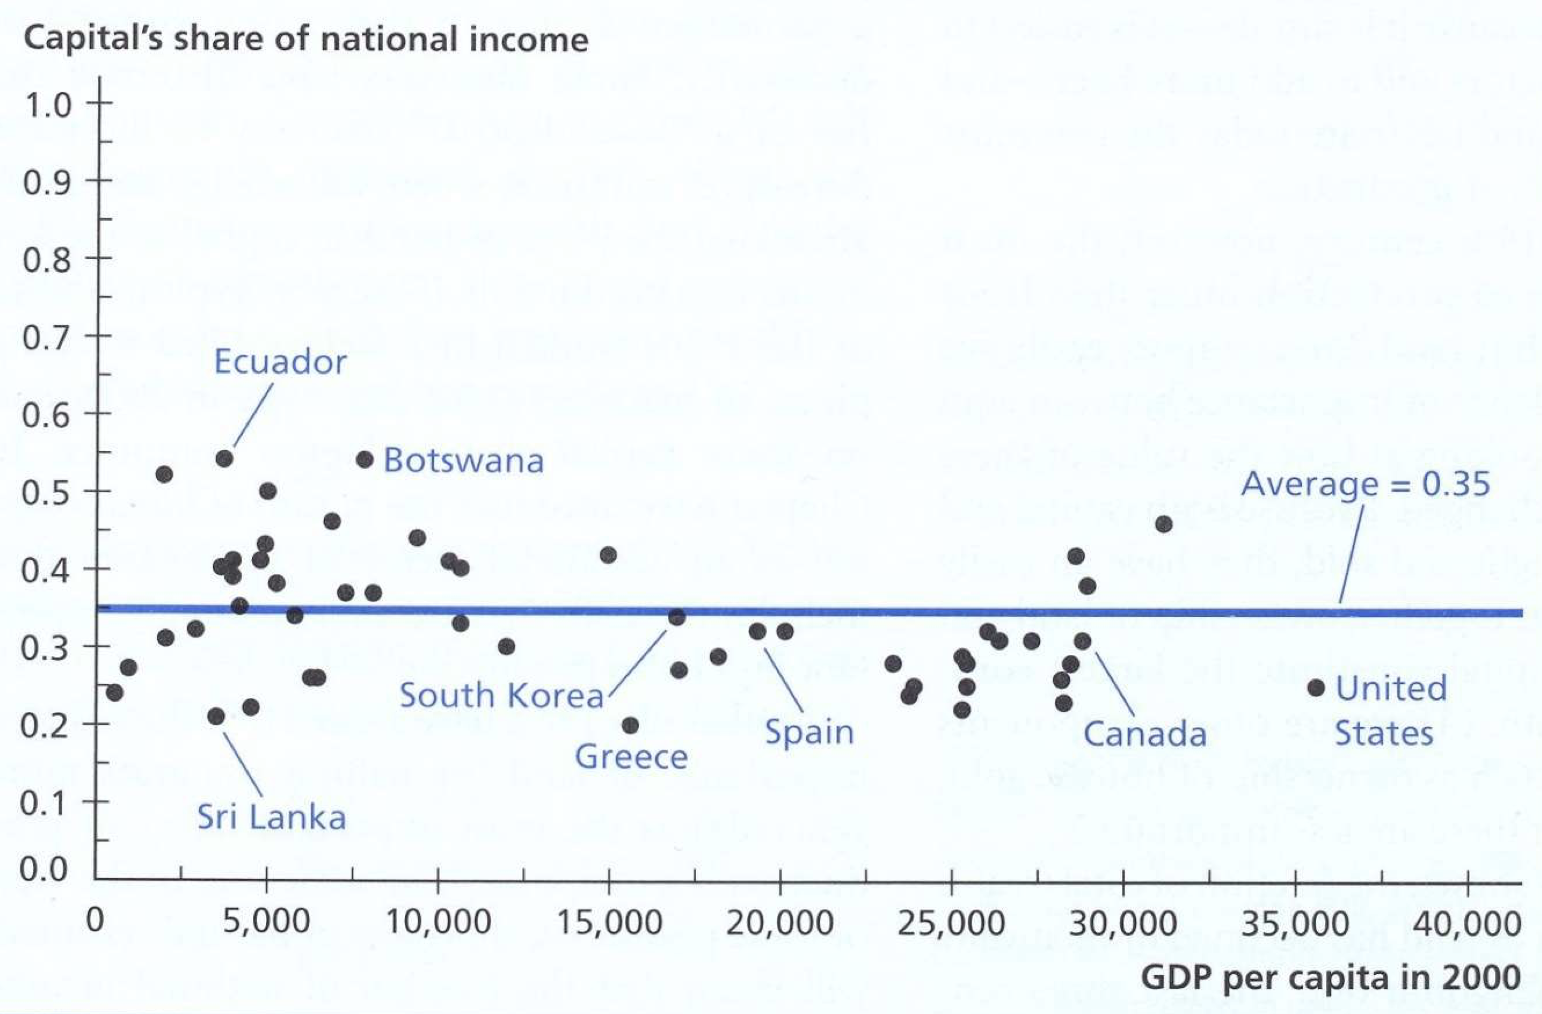
\includegraphics[width=0.4\linewidth]{capitalshare.png}
    \label{fig:placeholder}
\end{figure}

\end{tcolorbox}




\subsection{Market equilibrium and national income}
\textbf{Definition of general equilibrium:}\\\\
The general equilibrium consist of paths for quantities $[Y(t),K(t),a(t),C(t)]_{t=0}^{\infty}$ and prices $[w(t),r(t)]_{t=0}^{\infty}$, such that: 
\begin{itemize}
    \item Final good producers maximize profits $\pi = Y - wL - (r + \delta)K$ at each $t \in [0, \infty]$
    \item HH maximize life-time utility $U = \int_{0}^{\infty} u(C)e^{-\rho t}dt$
    \item Capital market clears, i.e. $a(t) = K(t)$ at each $t \in [0, \infty]$
    \item Labor market clears, i.e. $L^{S}(t) = L^{D}(t)$ at each $t \in [0, \infty]$
    \item Goods market clears, i.e. $Y(t) = I(t) + C(t)$ at each $t \in [0, \infty]$
\end{itemize}
\textbf{National income} $X$ equals aggregate production net of depreciation, which is shown here: 
\[
X = wL + rK = \underbrace{(1 - \alpha)\frac{Y}{L}}_{\text{$w$}} L + \underbrace{\left(\alpha\frac{Y}{K} - \delta\right)}_{\text{$r$}} K = Y - \delta K
\]
\subsubsection{Market equilibrium illustration}


\begin{figure}[H]
    \centering
    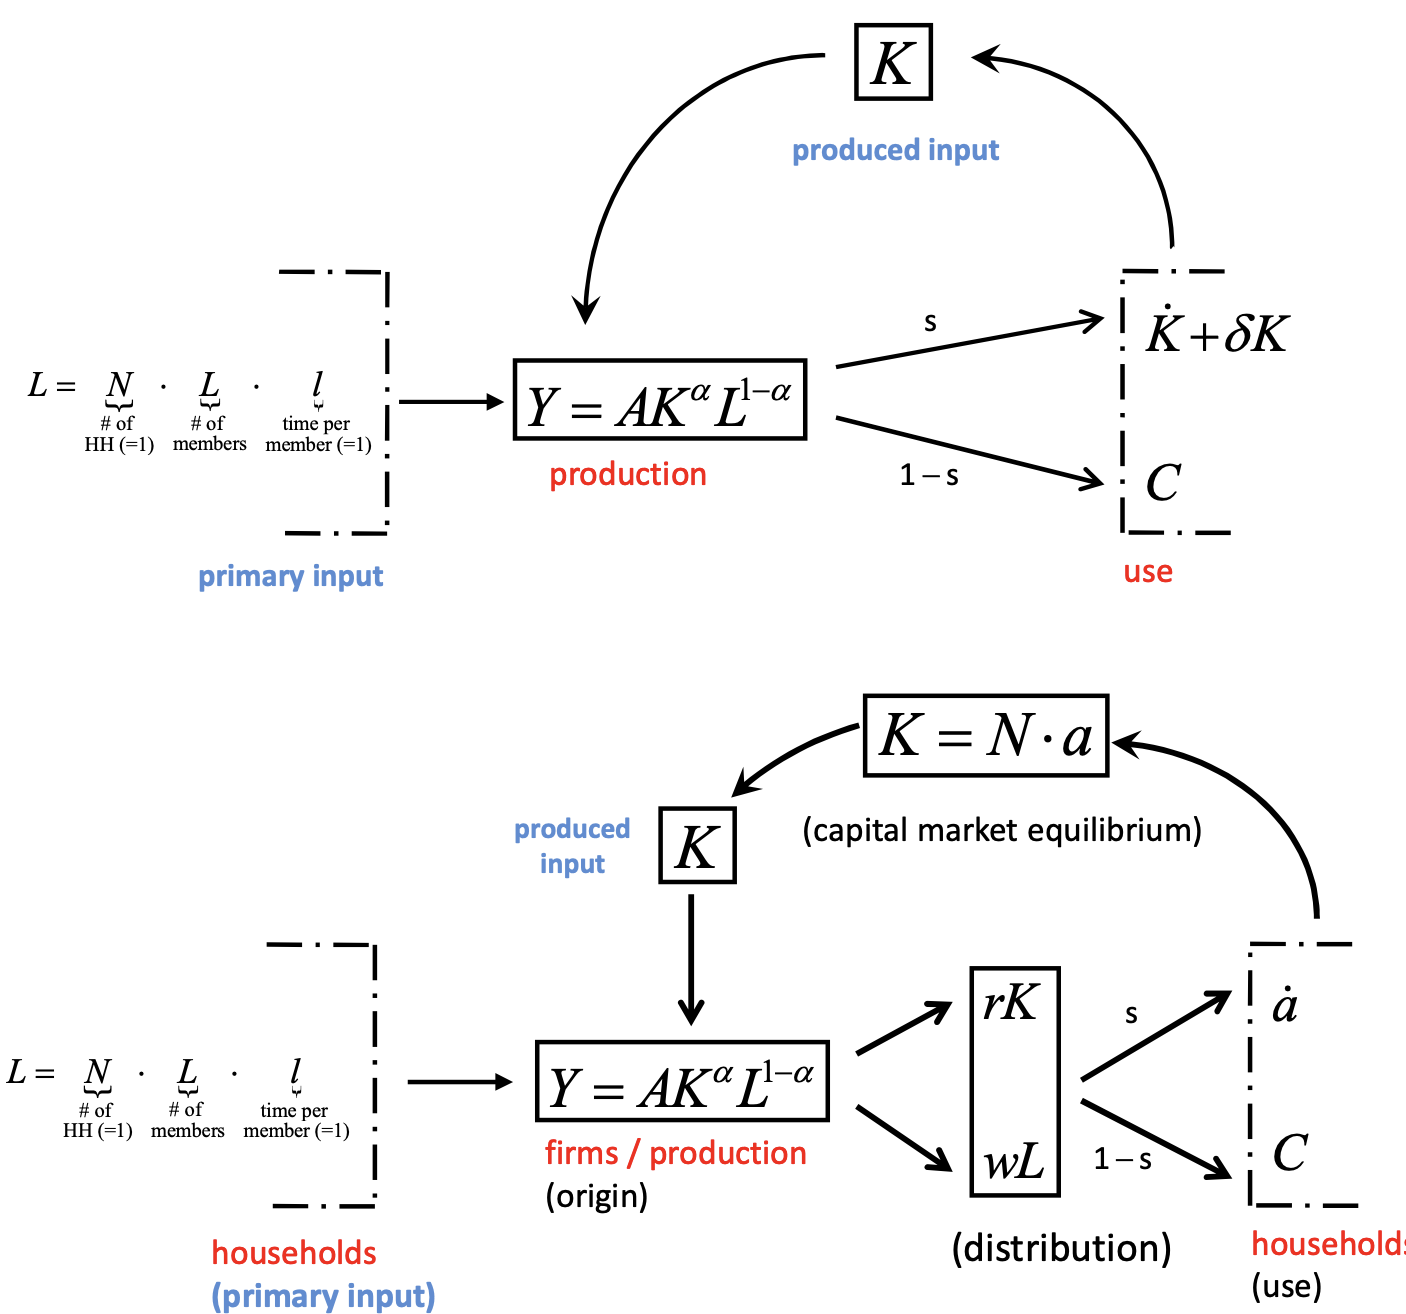
\includegraphics[width=0.5\linewidth]{dynamics.png}
\end{figure}
Interpretations: 
\begin{itemize}
    \item \textbf{Robinson-Crusoe economy:} Consumer-producer household accumulates output not consumed and thereby builds up a stock of physical capital. Stock of capital is used to produce output.
    \item \textbf{Market economy:} HH accumulate wealth (measured in terms of $Y$), which is rented out to firms. Firms employ this capital in the production of final output.
\end{itemize}

\subsection{Dynamics}
\begin{tcolorbox}[
    colback=red!5!white, % Very light red background (5% red, 95% white)
    colframe=red!40!white, % Light red border (30% red, 70% white)
    title=Definition: Steady State and Balanced Growth Path, % Optional title
    fonttitle=\bfseries % Bold title
]

A \textbf{\emph{steady state}} is a situation in which all relevant economic variables are constant over time, i.e., for any variable $x_t$, we have $x_{t+1} = x_t$ and $\dot{x}=0$. \\\\
A \textbf{\emph{balanced growth path}} is a situation in which the \textbf{growth rates} of all relevant economic variables are constant over time, i.e. $\hat{x}=const.>0$


\begin{itemize}
    \item A \emph{zero-growth steady state} is referred to simply as a \emph{steady state}.
    \item A \emph{positive-growth steady state} is referred to as a \emph{balanced growth path}.
\end{itemize}

\end{tcolorbox}



The dynamics of the economy are described by: 
$$\dot{C} = \frac{C}{\sigma}\left(\alpha K^{\alpha - 1} L^{1-\alpha} - \delta - \rho \right)$$
$$\dot{K} = K^{\alpha} L^{1-\alpha} - \delta K - C$$
Boundary condition: $K(0)=K_0$ and $C(\infty)=\tilde{C}$, whereas the second boundary condition substitutes the TVC\\\\

\begin{tcolorbox}[
    colback=blue!5!white, % Very light red background (5% red, 95% white)
    colframe=blue!40!white, % Light red border (30% red, 70% white)
    title=Derivation of the ODE system of the Ramsey model % Optional title
    ]
The system is derived by combining the household's optimization with the firm's production:

\textbf{1. The Consumption Euler Equation (KRR):}
The standard Keynes-Ramsey Rule for CRRA utility is:
$$\frac{\dot{C}}{C} = \frac{1}{\sigma}(r - \rho)$$
From the firm's FOC, we know the real interest rate is the marginal product of capital net of depreciation:\\ $r = \frac{\partial Y}{\partial K} - \delta = \alpha A K^{\alpha-1} L^{1-\alpha} - \delta$. Substituting this into the KRR:
$$\dot{C} = \frac{C}{\sigma} \left( \alpha K^{\alpha-1} L^{1-\alpha} - \delta - \rho \right)$$

\textbf{2. The Equation of Motion for Capital:}
From the aggregate resource constraint (Slide 71 logic):
\begin{enumerate}
    \item Output Identity: $Y = C + I$
    \item Capital Accumulation: $\dot{K} = I - \delta K$
    \item Production Function: $Y = K^{\alpha} L^{1-\alpha}$
\end{enumerate}
Combining these gives $\dot{K} = Y - C - \delta K$. Substituting the production function:
$$\dot{K} = K^{\alpha} L^{1-\alpha} - \delta K - C$$
$\dot{K}$ is defined to be net investment, we have: $\dot{K}=Y-C-\delta K$ \\
$\dot{K}+\delta K$ is defined to be gross investment, we have: $\dot{K}+\delta K=Y-C$
\begin{tcolorbox}[
    colback=blue!5!white, 
    colframe=black, 
    round corners, 
    boxrule=0.5pt,
    title=Alternative (market economy) version of the $\dot{K}$ equation,
    fonttitle=\bfseries,
    coltitle=black,
    attach title to upper
]
\vspace{0.5em} \\
Following the national accounting identities and budget constraints:
\begin{itemize}
    \item \textbf{Wealth Equilibrium:} $a(t) = K(t) \implies \dot{a}(t) = \dot{K}(t)$
    \item \textbf{Household Budget:} $\dot{a}(t) = w(t)L + r(t)a(t) - C(t)$
    \item \textbf{Accounting Identity:} Total factor income equals net output: 
    $w(t)L + r(t)K(t) = Y(t) - \delta K(t)$
\end{itemize}
Substituting the identity into the budget constraint gives:
$$\dot{K} = \underbrace{Y(t) - \delta K(t)}_{wL + rK} - C(t)$$
Plugging in the production function $Y = K^\alpha L^{1-\alpha}$:
$$\dot{K} = K^{\alpha} L^{1-\alpha} - \delta K - C$$
\end{tcolorbox}
\end{tcolorbox}
The zero-growth steady state is given by: 
$$\tilde{K} = \left(\frac{\alpha}{\delta + \rho}\right)^{\frac{1}{1-\alpha}} L \quad\quad\quad\quad \tilde{C} = \tilde{K}^{\alpha} L^{1-\alpha} - \delta \tilde{K}$$
\begin{tcolorbox}[
    colback=red!5!white, % Very light red background (5% red, 95% white)
    colframe=red!40!white, % Light red border (30% red, 70% white)
    title=Derivation of the steady state, % Optional title
    fonttitle=\bfseries % Bold title
    ]
The steady state $(\tilde{K}, \tilde{C})$ is found where the system dynamics settle $(\dot{K}=0, \dot{C}=0)$:

\textbf{1. The $\dot{K}=0$ Locus (Resource Constraint):}
Setting the capital motion equation to zero:
$$K^{\alpha} L^{1-\alpha} - \delta K - C = 0 \implies C = K^{\alpha} L^{1-\alpha} - \delta K$$
This is a hump-shaped curve in the $(K,C)$-plane, representing levels of consumption that keep capital constant.

\textbf{2. The $\dot{C}=0$ Locus (Euler Equation):}
Setting the consumption motion equation to zero:
$$\frac{C}{\sigma}(\alpha K^{\alpha - 1} L^{1-\alpha} - \delta - \rho) = 0$$
Ignoring the trivial case $C=0$, we solve for $K$:
$$\alpha K^{\alpha - 1} L^{1-\alpha} = \delta + \rho \implies K^{\alpha - 1} = \frac{\delta + \rho}{\alpha L^{1-\alpha}}$$
$$\tilde{K} = \left( \frac{\alpha}{\delta + \rho} \right)^{\frac{1}{1-\alpha}} L$$
This is a vertical line in the $(K,C)$-plane at $K = \tilde{K}$.

\textbf{3. Steady State Consumption:}
Substitute $\tilde{K}$ into the $\dot{K}=0$ equation:
$$\tilde{C} = \tilde{K}^{\alpha} L^{1-\alpha} - \delta \tilde{K}$$

\textbf{Extensions (Balanced Growth Path):}
If $L$ or $A$ grow, we define variables in efficiency units $k = \frac{K}{AL}$ and $c = \frac{C}{AL}$:
\begin{itemize}
    \item \textbf{With $L$ growth ($n$):} Replace $\delta$ with $(\delta + n)$ in the $\tilde{K}$ formula.
    \item \textbf{With $A$ growth ($g$):} Replace $\rho$ with $(\rho + \sigma g)$ and $\delta$ with $(\delta + n + g)$.
\end{itemize}
\end{tcolorbox}
\begin{tcolorbox}[
    colback=blue!5!white,
    colframe=blue!40!white,
    title=Typical errors with respect to steady state and balanced growth path,
    fonttitle=\bfseries
    ]

\textbf{1. Confusing steady state with BGP:}
A steady state ($\dot{x} = 0$) and a balanced growth path ($\hat{x} = \text{const.} > 0$) are not the same. A steady state is a \textit{special case} of a BGP where the constant growth rate happens to be zero.

\textbf{2. Assuming a steady state exists under technological progress:}
In models with technological progress ($\dot{A}/A = x > 0$), a classical steady state generally does not exist. Assuming $\tilde{K} = \text{const.}$ yields a contradiction, since the solution for $\tilde{K}$ depends on $AL$, which is growing.

\textbf{3. Forgetting what is constant in each concept:}
\begin{itemize}
    \item Steady state: the \textit{level} is constant ($\dot{x} = 0$)
    \item BGP: the \textit{growth rate} is constant ($\hat{x} = \text{const.} > 0$), while the level is still growing
\end{itemize}

\textbf{4. Skipping the proof when showing non-existance of a steady state}
The correct way to rule out a steady state is to assume it exists, derive what it implies, and show this leads to a contradiction - not to simply assert it does not exist.

\end{tcolorbox}



\subsection{Phase Diagram}

The phase diagram illustrates the uniqueness of the \textbf{Equilibrium Growth Path (EGP)}. It maps the joint dynamics of capital $K$ and consumption $C$ to show how the economy converges to a long-run equilibrium. The equilibrium growth path is characterized by the intersection of the $\dot{K}=0$ and $\dot{C}=0$. This yields the unique interior steady state (Point A), at which we have steady-state values $\tilde{C}$ and $\tilde{K}$.
\begin{figure}[H]
    \centering
    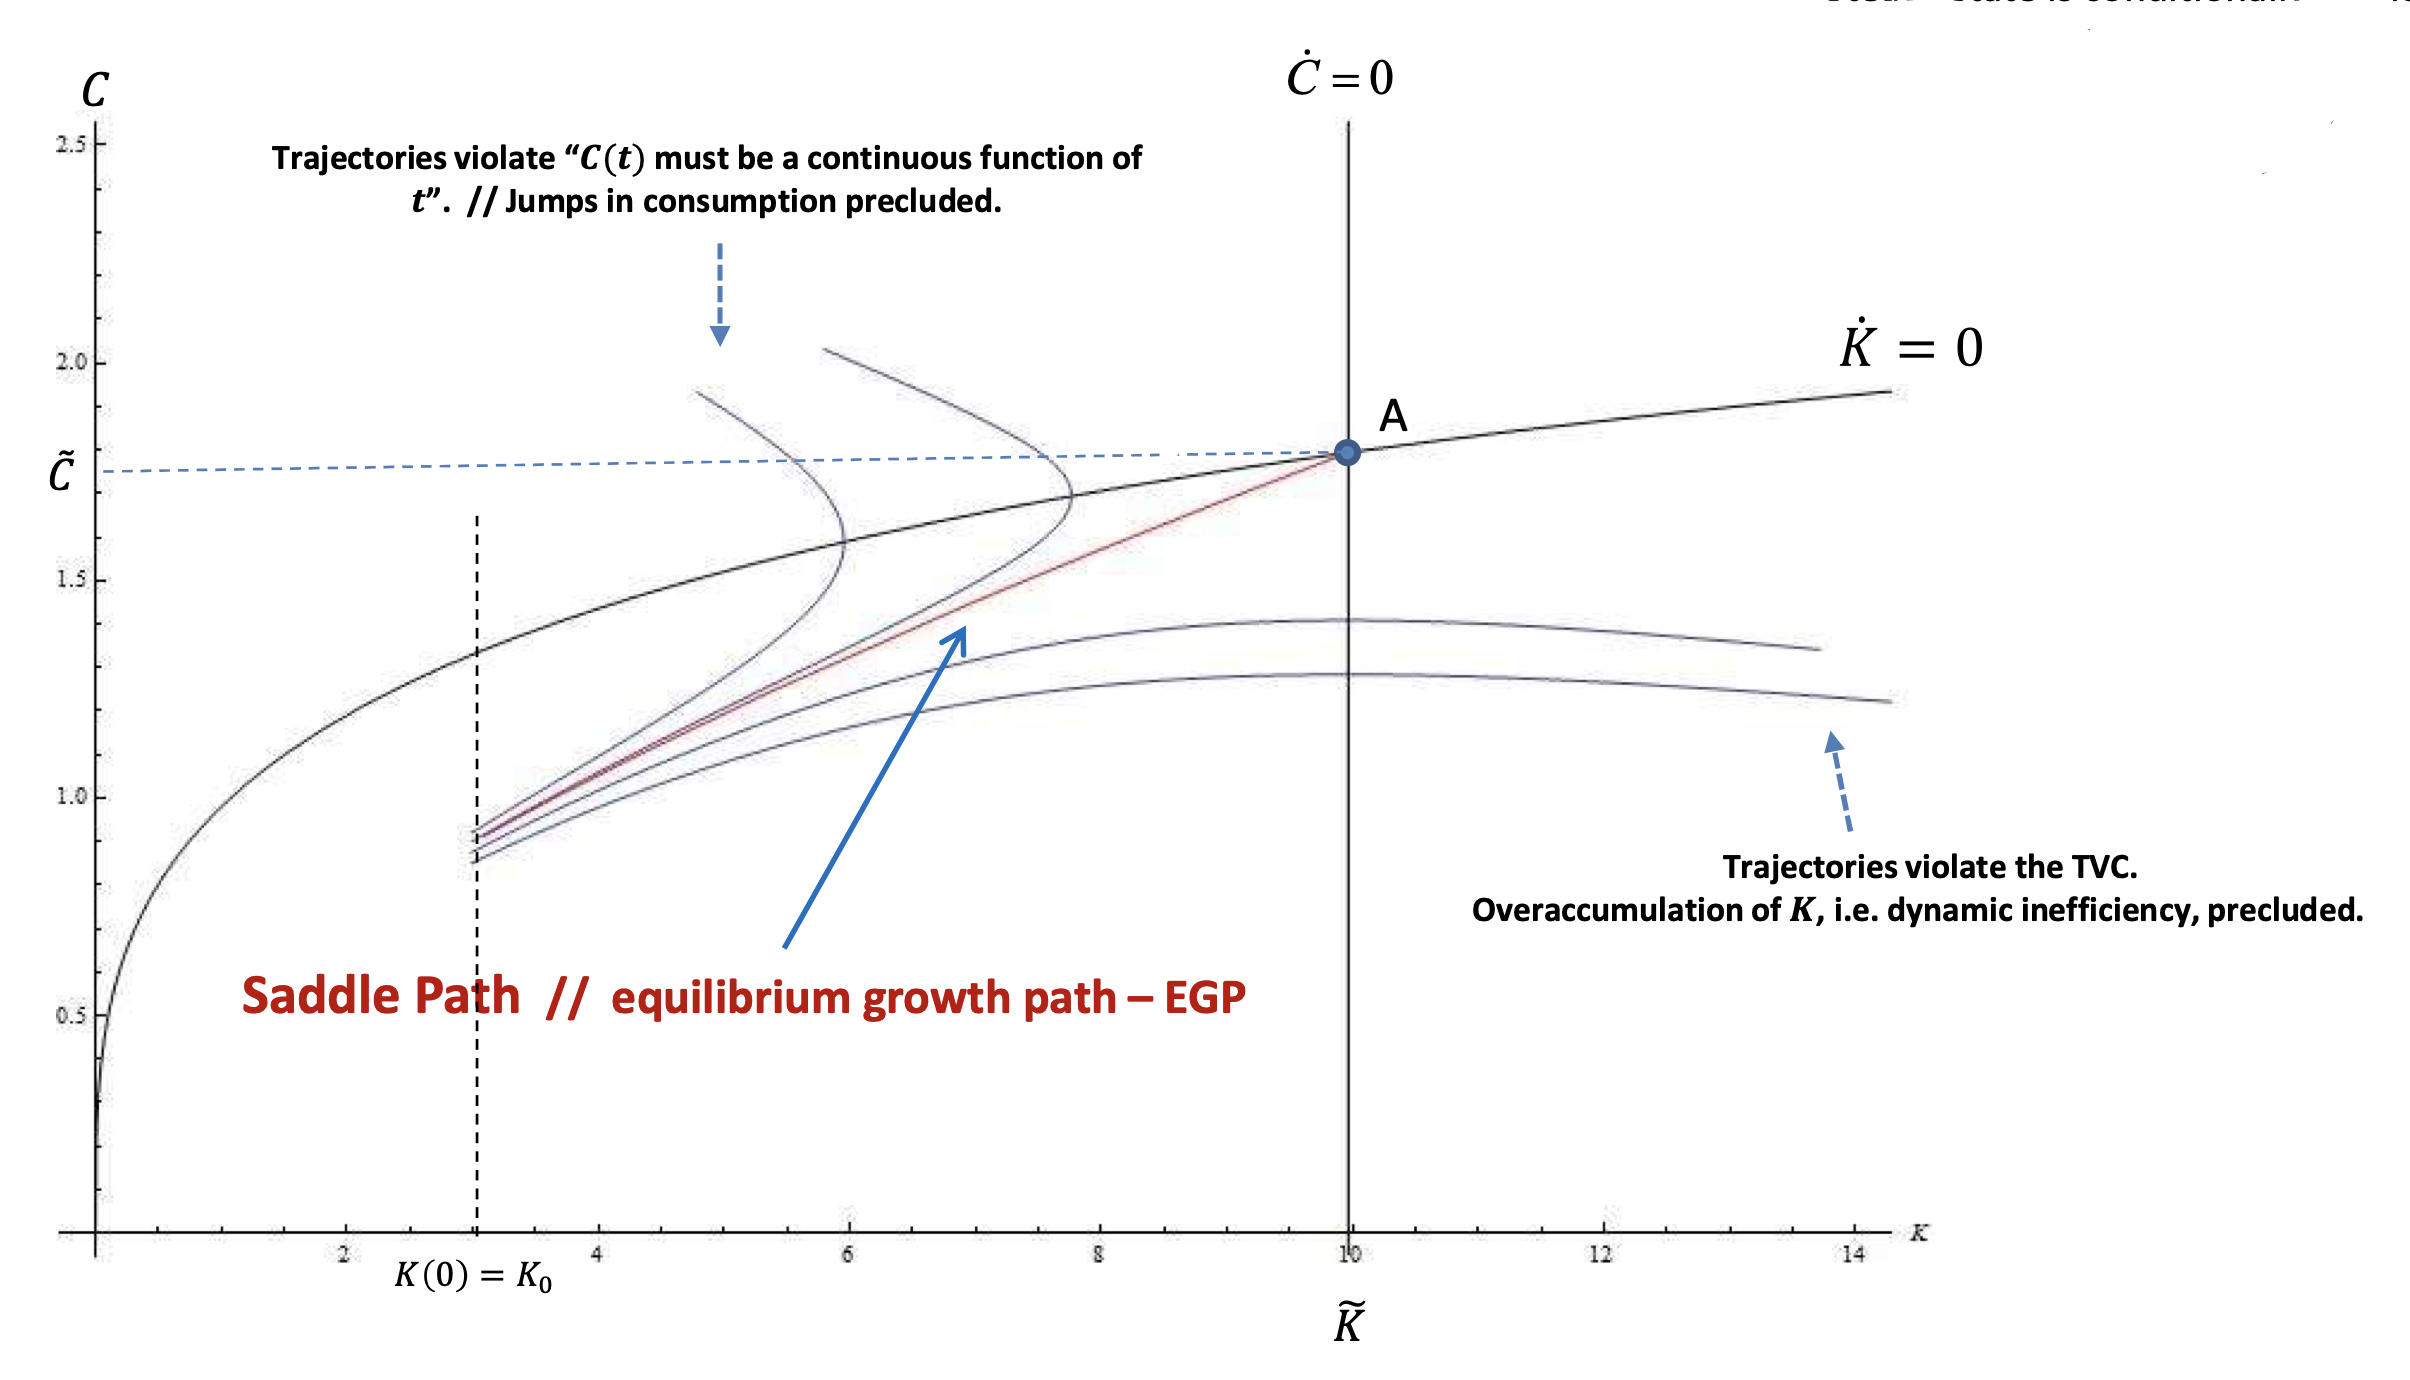
\includegraphics[width=0.7\linewidth]{phase.png}
    \caption{Phase Diagram of the Ramsey Model}
    \label{fig:phase_diagram}
\end{figure}

\begin{itemize}
    \item \textbf{Unique Initial Consumption:} Given a pre-determined initial capital stock $K(0) = K_0$, there is only one unique choice for initial consumption $C(0)$ such that the economy evolves along the unique EGP towards the steady state.
    \item \textbf{Saddle Point Stability:} The steady state is \textit{saddle point stable} (or conditionally stable). The system only converges if the initial $C(0)$ is chosen precisely on the stable manifold (the saddle path). Any initial value not on this path causes the system to diverge.
    \item \textbf{Divergence Paths and Boundary States:} The $\dot{K}=0$ locus is an inverted parabola starting at $(0,0)$ and ending at $(\bar{K}, 0)$, where $\bar{K}$ is the maximum sustainable capital stock. While $(0,0)$ and $(\bar{K},0)$ are technically steady states, they are ignored as they imply zero consumption.
    \item \textbf{Excessive Saving Logic:} If initial consumption $C(0)$ is set \textbf{too low} (below the saddle path), the household saves an excessive portion of its income. This leads to:
    \begin{enumerate}
        \item Rapid capital accumulation in the short run.
        \item Eventually, the marginal productivity of capital falls due to diminishing returns.
        \item Because the household is not consuming enough to satisfy the Transversality Condition (TVC), they continue to accumulate capital until it reaches the point $(\bar{K}, 0)$, where all production is used simply to replace depreciating capital ($\delta K = Y$), leaving nothing left for consumption. 
    \end{enumerate}
    \textit{Note: This path is ruled out by the household's optimization because it violates the Transversality Condition; it is not optimal to accumulate capital forever and never consume it.}
\end{itemize}
\begin{tcolorbox}[
    colback=blue!1!white,
    colframe=blue!40!white,
    title=Why Exactly One Trajectory? Ruling Out All Others,
    fonttitle=\bfseries
    ]
The phase diagram contains \textit{infinitely many} trajectories starting from $K_0$, but only \textbf{one} survives the household's optimality conditions. The argument has two parts: trajectories \textbf{above} the saddle path are ruled out by the TVC, trajectories \textbf{below} the saddle path are ruled out either by the TVC or by feasibility.

\textit{Trajectories above the saddle path (initial $C(0)$ too high).}
\begin{itemize}
    \item Initial consumption is so high that the household consumes more than what is sustainable. Capital is run down (or grows too slowly) while consumption keeps rising.
    \item The trajectory crosses the $\dot K = 0$ locus and heads toward the $C$-axis: $K \to 0$, $C$ keeps rising.
    \item At some finite time, $K$ hits zero and $C$ would have to jump down discontinuously, since with no capital there is no production. \textbf{This violates the requirement that $C(t)$ be a continuous function of time} (jumps in consumption are precluded by the optimization).
    \item Equivalently: the present-value shadow price of wealth $e^{-\rho t}\lambda(t) a(t)$ becomes negative or fails to converge to zero, violating the TVC.
\end{itemize}

\textit{Trajectories below the saddle path (initial $C(0)$ too low).}
\begin{itemize}
    \item The household saves an excessive portion of income. Capital accumulates rapidly while consumption stays low.
    \item Eventually the marginal product of capital falls below $\rho + \delta$ due to diminishing returns. The economy is now in the \textbf{dynamically inefficient region}: it accumulates capital that yields lower returns than what discounting demands.
    \item The trajectory drifts toward $(\bar K, 0)$, where all output is used to replace depreciation ($\delta K = Y$) and consumption is permanently zero.
    \item Although feasible, this path \textbf{violates the TVC}: $\lim_{t\to\infty} e^{-\rho t}\lambda(t) a(t) > 0$, meaning the household dies with positive wealth. Lifetime utility could be raised by consuming more, so this path is not optimal.
\end{itemize}
\textit{Optimal unique $C(0)$.}
\begin{itemize}
    \item Only the saddle path satisfies (i) continuity of $C(t)$, (ii) feasibility ($K \geq 0$ at all times), and (iii) the TVC. This pins down a unique $C(0)$ for any given $K_0$. The saddle path is therefore the \textbf{balanced growth path}: the household's optimization \textit{selects} it from the continuum of feasible trajectories.
    \item \textit{Mathematical reason:} Linearizing the dynamic system around the steady state yields two eigenvalues of opposite sign ($\mu_1 < 0 < \mu_2$). The general solution is $z(t) = \alpha_1 e^{\mu_1 t} v_1 + \alpha_2 e^{\mu_2 t} v_2$. The TVC forces $\alpha_2 = 0$ (otherwise the unstable mode explodes), and $\alpha_1$ is then pinned down by the initial condition $K(0) = K_0$. Saddle-path stability is thus a direct consequence of having one predetermined state ($K$) and one free jump variable ($C$).
\end{itemize}
\end{tcolorbox}

\begin{tcolorbox}[
    colback=blue!5!white, % Very light red background (5% red, 95% white)
    colframe=blue!40!white, % Light red border (30% red, 70% white)
    title=Numerical solution of the Ramsey model
    ]
Numerical solution of the Ramsey model with the following differential equations:
$$\dot{k}(t) = k(t)^\alpha - \delta\, k(t) - c(t)$$
$$\dot{c}(t) = c(t)\,\bigl[\alpha\, k(t)^{\alpha-1} - \delta - \rho\bigr]$$

\begin{figure}[H]
    \centering
    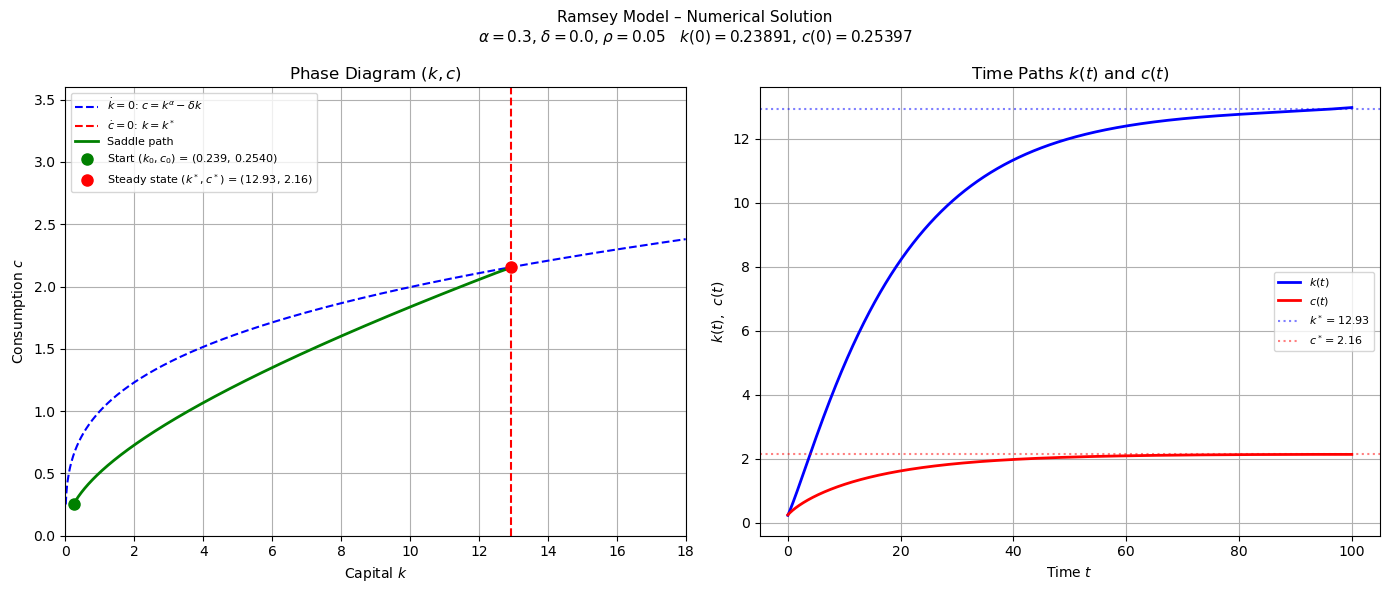
\includegraphics[width=1\linewidth]{ramseynum.png}
    \label{fig:placeholder}
\end{figure}
\end{tcolorbox}


\subsection{Social planner's solution}
Social planner maximizes life-time utility of typical household by solving: 
$$\max_{\{C\}} \int_{0}^{\infty} \frac{C^{1-\sigma} - 1}{1-\sigma} e^{-\rho t}\, dt$$
$$\text{s.t. } \dot{K} = K^{\alpha} L^{1-\alpha} - \delta K - C$$
$$K(0) = K_0,\; K(t) \ge 0$$
The equation for $\dot{K}$ results from the resource constraint $Y-\delta K=\dot{K}+C$ \\\\
\textbf{Setting up the Hamiltonian} for this problem gives us: 
\[ H := \frac{C^{1-\sigma} - 1}{1 - \sigma} + \mu (K^{\alpha} L^{1-\alpha} - \delta K - C) \]

\[ H_{C} = C^{-\sigma} - \mu = 0 \]

\[ \dot{\mu} = -H_{K} + \rho \mu = -\mu \alpha K^{\alpha-1} L^{1-\alpha} + \mu \delta + \rho \mu \]\\\\
\textbf{The implied Keynes-Ramsey-Rule} is: 
\[ \frac{\dot{C}}{C} = \frac{1}{\sigma} \left( \alpha K^{\alpha-1} L^{1-\alpha} - \delta - \rho \right)\]\\\\
The \textbf{evolution of the economy} is \textbf{determined} by the \textbf{KKR}, the \textbf{flow budget constraint} $(\dot{K} = K^{\alpha} L^{1-\alpha} - \delta K - C)$ and the \textbf{initial} and \textbf{boundary} \textbf{conditions} $(K(0)=K_0, \quad C(\infty)=\tilde{C})$\\\\
\textbf{Important Implications:}
\begin{itemize}
    \item Decentralized equilibrium aligns with the social planner’s solution, meaning the \textbf{market equilibrium is the unique first-best outcome}.

\item This result stems from the assumption of a \textbf{perfectly neoclassical economy} ($\rightarrow$ First theorem of welfare economics states that any competitive equilibrium is Pareto-efficient).
\end{itemize}



\subsection{Technological progress}
The following notation employs a \textbf{exogenous} and \textbf{labor augmenting} production function: 
$$Y=K^\alpha(AL)^{1-\alpha} \quad \quad with \quad A=A_0e^{xt},x\geq0$$
Following the same steps (setting up the Hamiltonian and solving for the KKR) yields a very similar \textbf{dynamic system to describe the economy}:
\begin{equation}
    \dot{C} = \frac{C}{\sigma} \left( \alpha K^{\alpha-1} (AL)^{1-\alpha} - \delta - \rho \right)
    \label{KRR1.6}
\end{equation}
\begin{equation}
    \dot{K} = K^{\alpha} (AL)^{1-\alpha} - \delta K - C
    \label{Kdot1.6}
\end{equation}
\begin{tcolorbox}[
    colback=red!5!white, % Very light red background (5% red, 95% white)
    colframe=red!40!white, % Light red border (30% red, 70% white)
    title=Derivation: Steady state with labor-augmenting endogenous technological advancement, % Optional title
    fonttitle=\bfseries % Bold title
    ]
    We consider the growth rates of $C$ and $K$, using equations \eqref{KRR1.6} and \eqref{Kdot1.6}: \\
    $$\hat{C} &= \frac{\textcolor{red}{\alpha K^{\alpha-1}(AL)^{1-\alpha}} - \delta - \rho}{\sigma}$$
    $$\hat{K} &= \underbrace{K^{\alpha-1}(AL)^{1-\alpha}}_{\textcolor{blue}{Y/K}} - \delta - \textcolor{blue}{C/K}$$\\
    Consider the RHS of $\hat{C}$: Only $\alpha K^{\alpha-1}(AL)^{1-\alpha}$ changes over time, taking growth rates (by ln-differentiating) and setting such equal to zero gives: $(\alpha-1)\hat{K}+(1-\alpha)\hat{A}=0\quad \Leftrightarrow \quad \hat{K}=\hat{A}$\\
    Consider the RHS of $\hat{K}:$ We know that $\hat{K}=\hat{A}$ leads to $\alpha K^{\alpha-1}(AL)^{1-\alpha}=const.$, thus $K^{\alpha-1}(AL)^{1-\alpha}=Y/K=const.$.\\
    Now for $C/K$ to best $const.$ it must be that $\hat{C}=\hat{K}$.\\\\
    In summary we get: $\hat{Y}^*=\hat{K}^*=\hat{C}^*=\hat{A}^*=x$, whereas $x$ is the growth rate of $\hat{A}$ by construction. \\\\
    Note: With labor growth (i.e. growing population) we'd have $\hat{Y}=\hat{L}+\hat{A}=n+x$
\end{tcolorbox}
\subsubsection{Normalization of variables}
We transform variables so that a dynamics system turns into system that converges towards a stationary solution:
 Let $X(t)$ be a variable that grows in the long run at rate $g$, the normalized variable is given by $x(t)=X(t)/e^{gt}$. This yields, by construction, $lim_{t\to\infty}x(t)=const.$\\\\
For the model above the normalization works as follows: 
$$c : = \frac{\color{red}C}{e^{(x+n)t}} = \frac{C}{AL} \quad \text{and} \quad k := \frac{\color{black!60!black}K}{e^{(x+n)t}} = \frac{K}{AL}$$
This transformation 'removes' the growth rate of labor $n$ and technological progress $x$ from our variables: $\hat{c}=\hat{C}-\hat{L}-\hat{A}=0$ and  $\hat{k}=\hat{K}-\hat{L}-\hat{A}=0$\\\\
The dynamics system described by \eqref{Kdot1.6} and \eqref{KRR1.6} in normalized variables: 
$$\dot{c} = \frac{c}{\sigma} \left[ \alpha k^{\alpha-1} - (\delta + \rho + x \sigma) \right]$$

$$\dot{k} = k^{\alpha} - c - (x + \delta)k$$





\subsection{Overview of cases and tasks for the Ramsey model}
\renewcommand{\arraystretch}{1.4} % mehr vertikaler Abstand
\setlength{\tabcolsep}{10pt}     % mehr horizontaler Abstand
\setlength{\arrayrulewidth}{0.4pt} % dünnere Linien


\renewcommand{\arraystretch}{1.4}
\setlength{\tabcolsep}{10pt}
\setlength{\arrayrulewidth}{0.4pt}
\begin{table}[h!]
\centering
\resizebox{\textwidth}{!}{
\begin{tabular}{lccc}
\hline
 & No growth & Population growth ($n>0$) & Pop.\ \& tech growth ($n>0, x>0$) \\
\hline
Aggregate variables
& $Y, K, C, L$
& $Y, K, C, L$
& $Y, K, C, L$ \\
\hline
Intensive variables
& ---
& $y = \frac{Y}{L},\ k = \frac{K}{L},\ c = \frac{C}{L}$
& $\tilde{y} = \frac{Y}{AL},\ \tilde{k} = \frac{K}{AL},\ \tilde{c} = \frac{C}{AL}$ \\
\hline
Output
& $Y = K^\alpha L^{1-\alpha}$
& $y = k^\alpha$
& $\tilde{y} = \tilde{k}^\alpha$ \\
\hline
Resource constraint 
& $\dot{K} = K^\alpha L^{1-\alpha} - \delta K - C$ 
& $\dot{k} = k^\alpha - (n+\delta)k - c$ 
& $\dot{\tilde{k}} = \tilde{k}^\alpha - (n+x+\delta)\tilde{k} - \tilde{c}$ \\
\hline
Euler equation 
& $\frac{\dot{C}}{C} = \frac{1}{\sigma}(\alpha K^{\alpha-1}L^{1-\alpha}-\delta-\rho)$ 
& $\frac{\dot{c}}{c} = \frac{1}{\sigma}(\alpha k^{\alpha-1}-\delta-\rho)$ 
& $\frac{\dot{\tilde{c}}}{\tilde{c}} = \frac{1}{\sigma}(\alpha\tilde{k}^{\alpha-1}-\delta-\rho - \sigma x)$ \\
\hline
Steady state condition 
& $\alpha K^{*\,\alpha-1} L^{1-\alpha} = \delta + \rho$ 
& $\alpha k^{*\,\alpha-1} = \delta + \rho$ 
& $\alpha \tilde{k}^{*\,\alpha-1} = \delta + \rho + \sigma x$ \\
\hline
Growth rates (SS) 
& $\hat{Y}^* = \hat{K}^* = \hat{C}^* = 0$ 
& $\hat{Y}^* = \hat{K}^* = \hat{C}^* = n$ 
& $\hat{Y}^* = \hat{K}^* = \hat{C}^* = n+x$ \\
\hline
Growth rates per capita (SS)
& $\widehat{(Y/L)}^* = \widehat{(C/L)}^* = 0$
& $\widehat{(Y/L)}^* = \widehat{(C/L)}^* = 0$
& $\widehat{(Y/L)}^* = \widehat{(C/L)}^* = x$ \\
\hline
\end{tabular}
}
\caption{Overview of Ramsey model cases with Cobb-Douglas production $Y = K^\alpha L^{1-\alpha}$. In the no growth case $L = \text{const.}$, so no normalization is needed. In columns 2 and 3, variables are normalized by $L$ and $AL$ respectively. The steady state conditions follow from setting the Euler equation to zero and using $r = \alpha k^{\alpha - 1}$.}
\end{table}